\documentclass[11pt]{article}
\usepackage[margin=1in]{geometry}
\usepackage{amsmath,amssymb,amsthm}
\usepackage{alltt}
\usepackage{graphicx}
\usepackage[T1]{fontenc}
\usepackage{lmodern}
\usepackage[colorlinks=true,linkcolor=blue,citecolor=blue,urlcolor=blue]{hyperref}
\hypersetup{pdftitle={The Thomson problem for N = 10},pdfauthor={P. Graham}}
\newtheorem{theorem}{Theorem}
\newtheorem{lemma}{Lemma}
\newcommand{\R}{\mathbb{R}}
\newcommand{\E}{\mathcal{E}}
\title{The Thomson problem for N = 10}
\author{P. Graham\\ \small\url{https://orcid.org/0009-0007-8493-1505}}
\date{October 22, 2026}
\begin{document}
\maketitle
\begin{abstract}
Thomson's problem, originating in his 1904 atomic model, asks for the least
Coulomb energy of points on a sphere. For $N = 10$ distinct points on the unit
sphere in $\R^3$, we prove that the energy
$\sum_{i<j}\|x_i-x_j\|^{-1}$ is minimized uniquely, up to orthogonal maps
and relabeling, by the $D_{4d}$ bicapped square antiprism. Its height
parameter is the distance of either square from the equatorial plane.
The chosen height is the unique critical point of the energy in a
specified exact interval. Adapting the nine-point proof design,
the proof first confines the inner products of every
competitor of no greater energy to seven small intervals. Classifying
the possible interval patterns and aligning the configurations then
reduces the problem to a quantitative local energy inequality that
forces equality with the candidate. The computer-assisted proof is
formally verified in Lean.
\end{abstract}

The proofs, the Lean formalization, the certificate checkers and the text
were produced by AI models (from OpenAI and Anthropic), working under the
author's direction.

\section{Introduction}
Thomson's problem asks for the least Coulomb energy of $N$ distinct unit
vectors in three dimensions. The problem originates in Thomson's 1904
atomic model~\cite{thomson}. For $N = 10$ charges, the familiar candidate has
two poles and two squares at opposite heights, rotated by $\pi/4$
relative to one another (Figure~\ref{fig:antiprism}). Their height is approximately $0.4226874$ and
the energy is approximately $32.71694946$. We prove that this $D_{4d}$
bicapped square antiprism is the unique global minimizer, up to orthogonal maps and
relabeling; Theorem~\ref{thm:main} gives the exact statement. No symmetry is assumed of competitors.

Optimizing within this one-parameter family does not settle the global
problem: competitors may have no symmetry. The main task is to localize
all such competitors. The two-point bound used here is only about
$32.66696$, below the candidate energy, so it cannot establish optimality.
Its role is to separate points. A three-point bound then puts every
competitor's energy above the candidate energy minus $10^{-30}$ whenever
all distinct pair inner products are at most $13/20$. The hard step is to turn this small energy error into
control of every competitor's geometry. The window classification does
this; the local energy inequality removes the error entirely.

The proof has four steps. First, a two-point bound separates distinct
points, after which a polynomial lower bound for pair energy and a
three-point energy estimate force all pairwise inner products of a
competitor of no greater energy into seven small intervals around the
candidate's inner products. Second, a finite classification shows that
these intervals can occur on the pairs in only the candidate's pattern,
up to relabeling. Third, an orthogonal alignment converts this control of
inner products into a bound on the point displacements. Finally, the
height equation and symmetry give full spherical stationarity, and a
positive second variation, together with a bound on the higher-order
error, makes every sufficiently small nonzero aligned displacement
increase the energy. This last step turns approximate localization into
exact equality.

The argument builds directly on the nine-point proof published by
Aravind Karthigeyan, which Anthropic's Opus 5.5 and OpenAI's GPT-6 Astra
generated under his direction and which, unreviewed, he released
requesting external review~\cite{n9}, including substantial reuse of its
MIT-licensed Lean code. For the ten-point geometry we supply new
energy, window-classification and Hessian certificates. The formal proof covers optimality, every equality
case and the fact that the candidate consists of distinct unit vectors.
To our knowledge no earlier rigorous proof for $N=10$ exists, and we make
no priority claim. Concurrent ten-point Lean proofs establish local
minimality and a long-chord condition~\cite{concurrent}; neither asserts
global optimality. The prior exact cases and these concurrent results
are described in Section~\ref{sec:prior}. Neither the present work nor
the nine-point work is yet peer-reviewed.
The theorem includes uniqueness, and its Lean verification is a formal
proof. Being the first rigorous proof or the first formal proof is a
historical claim, subject to the qualification just stated.

\paragraph{What is new beyond nine points.}
The proof follows the design of the nine-point project step by step and
reuses most of its Lean code: the form of the statement, the three-point
bound with its certificate checks, the Bernstein checks
of one-variable inequalities, the interval tests of the window
classification, the orthogonal alignment, the higher-order error bound and
the interval method for the Hessian. As it stood, that machinery did not
reach ten points in three places. First, a three-point certificate belongs
to one configuration, and we needed one that is sharp at the antiprism, so
that it misses the candidate energy by less than $10^{-30}$. Second, the
nine-point classification excludes inner products near $-1$ by a
Gram-determinant estimate and works with six windows. Here the poles are
antipodal, so $-1$ is a genuine seventh window, and the two poles with two
opposite points of a square lie in one plane through the origin. Every
triangle among those four points is then degenerate, so the nine-point
proof that four points always contain an anchor triple fails; a counting
argument over five points replaces it (Section~\ref{sec:global}). Third,
the local bound certifies one matrix. The ten-point Hessian is
$30\times30$, and its smallest eigenvalue transverse to rotations is about
$0.096$, against about $0.144$ for nine points, so the shift, the radius
and the interval data are new, as is the stationarity calculation for the
$D_{4d}$ symmetry. The first of the three was the hardest. A numerical
semidefinite solution is far less accurate than $10^{-30}$; our
certificate rounds, to rationals with denominator $2^{200}$, an exact
three-point certificate that is sharp for ten points, whose one-variable
polynomial touches the pair potential at $-1$ and at the six other
candidate inner products.

Section~\ref{sec:candidate} defines the candidate and states the theorem.
Section~\ref{sec:global} proves the two global localization steps;
Section~\ref{sec:local} completes the argument by alignment and local
rigidity. The separate numerical energy enclosure follows the theorem, and
Section~\ref{sec:prior} records the prior and concurrent work. Appendix~\ref{app:formal} supplies the exact parameter interval,
formal declarations, certificate sizes and checking requirements. The
text explains the mathematical reductions; the accompanying Lean proof
checks the rational inequalities and finite classifications they use.

\section{Statement and candidate}\label{sec:candidate}
This section specifies the configuration and the exact optimization
problem. Every competitor consists of ten distinct unit vectors.
For an injective map $x:\{0,\ldots,9\}\to S^2\subset\R^3$, put
\[
  \E(x)=\sum_{0\leq i<j\leq9}\frac1{\|x_i-x_j\|}.
\]
We call two configurations congruent when one is obtained from the other
by an element of $O(3)$ and a permutation of the ten indices; reflections
are allowed.

For $0<h<1$, write $r=\sqrt{1-h^2}$ and $q=r/\sqrt2$. Define $p(h)$ by
\begin{align*}
 p_0&=(0,0,1),&p_1&=(0,0,-1),\\
 p_2&=(r,0,h),&p_3&=(0,r,h),&p_4&=(-r,0,h),&p_5&=(0,-r,h),\\
 p_6&=(q,q,-h),&p_7&=(-q,q,-h),&p_8&=(-q,-q,-h),&p_9&=(q,-q,-h).
\end{align*}
These coordinates are preserved by rotation through $\pi/4$ about the
polar axis followed by reflection in the equatorial plane, and by
reflection in the vertical plane through $p_2$ and the poles. The
16-element group generated by these maps is conventionally denoted
$D_{4d}$.

\begin{figure}[t]
\centering
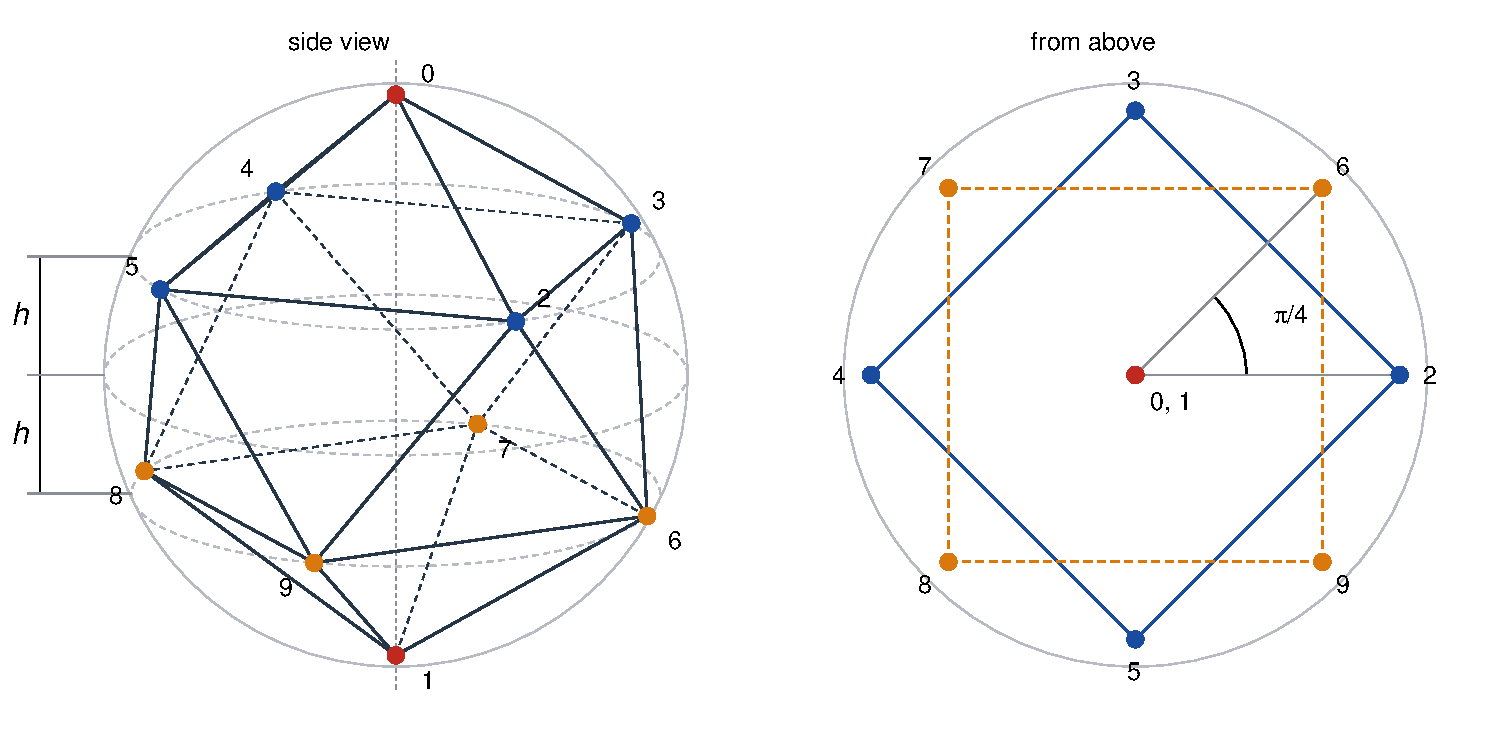
\includegraphics[width=\linewidth]{../data/antiprism.pdf}
\caption{The candidate $p(h_*)$. Left: a side view of the ten points and
the edges of their convex hull, hidden edges dashed. The poles $p_0,p_1$
are red, the upper square $p_2,\ldots,p_5$ at height $h=h_*$ is blue, and
the lower square $p_6,\ldots,p_9$ at height $-h$ is orange; the dashed
ellipses are the equator and the two circles of latitude. Right: the view
from above, in which the lower square (dashed) is the upper square rotated
by $\pi/4$. A label $i$ marks $p_i$. The figure is drawn from the Lean
definition of the candidate by \nolinkurl{checks/draw_antiprism.py}, which
checks that the drawn points are the candidate's; it is not part of the
proof.}
\label{fig:antiprism}
\end{figure}
The 45 unordered pairs consist of one pole pair, eight neighboring and
four opposite pairs within the squares, two classes of eight pairs
between the squares, and sixteen pole--square pairs. Grouping them gives
\begin{align}
 F(h)={}&\frac12+\frac{4\sqrt2+2}{\sqrt{1-h^2}}
 +\frac8{\sqrt{2-\sqrt2+(2+\sqrt2)h^2}}
 +\frac8{\sqrt{2+\sqrt2+(2-\sqrt2)h^2}}\nonumber\\
 &+\frac8{\sqrt{2-2h}}+\frac8{\sqrt{2+2h}}.\label{eq:energy}
\end{align}
The terms appear in that order: pole pair, pairs within the squares,
the two between-square classes, and the two pole--square classes.
Write $S(h)=F'(h)$ for the derivative of this energy with respect to
height. Its explicit formula is given in Appendix~\ref{app:interval}.
Let $[a,b]$ be the exact rational interval specified in
Appendix~\ref{app:interval}. It satisfies $0<a<b<1$ and
$b-a=1/(2D)<2^{-300}$, where the integer denominator $D$ is given there.
For orientation, this narrow interval lies inside
\[ [0.42268742404398,0.42268742404400]. \]
The derivative $S$ is continuous and strictly increasing on $[a,b]$,
and its endpoint signs satisfy $S(a)<0<S(b)$. The intermediate value
theorem and strict monotonicity therefore give a unique zero in this
interval. Define $h_*$ by $S(h_*)=0$ and $h_*\in[a,b]$.
Its decimal begins $0.422687424043986\ldots$. The root existence and
uniqueness in this specified interval are proved in Lean. This interval
selects the candidate; the global theorem still compares it with every
admissible configuration, including all other heights.

\begin{theorem}\label{thm:main}
The parameter $h_*$ exists and is unique in $[a,b]$. The configuration
$p=p(h_*)$ consists of ten distinct points on $S^2$. For every injective
$x:\{0,\ldots,9\}\to S^2$,
\[
 \E(p)\leq\E(x),\qquad
 \E(x)=\E(p)\quad\Longleftrightarrow\quad
 \exists Q\in O(3),\ \exists\sigma\in S_{10},\
 x_i=Qp_{\sigma(i)}\ \text{for all }i.
\]
\end{theorem}

Here and below, admissibility means precisely unit norm and injectivity.
The candidate is admissible: in the coordinates above, unit norm follows
from $r^2=1-h_*^2$ and $2q^2=r^2$. The two poles and the two squares
have distinct heights; within each square the four planar coordinates
are distinct because $r,q>0$. Thus the ten points are distinct. Appendix~\ref{app:statements} identifies the formal statements
of both the optimization theorem and this candidate-validity assertion.

The seven distinct inner products of the candidate are
\[
 -1,\quad h_*,\quad-h_*,\quad h_*^2,\quad2h_*^2-1,\quad
 \frac{1-h_*^2}{\sqrt2}-h_*^2,\quad
 -\frac{1-h_*^2}{\sqrt2}-h_*^2.
\]
\paragraph{Remark (energy enclosure).}\label{sec:energy}
A separate rigorous evaluation of the candidate energy gives
\[
 32.716949460147<\E(p)<32.716949460149,
\]
so the energy starts $32.71694946\ldots$. This rigorous rational-interval
computation is separate from the formal theorem. Appendix~\ref{app:energy}
gives the independent Python calculation and its exact inputs.

\section{From energy bounds to a common interval pattern}\label{sec:global}
We now show that every admissible competitor of energy at most the
candidate's has nearly the same matrix of pairwise inner products, after
relabeling. Let $f(t)=(2-2t)^{-1/2}$. For unit vectors, the pair energy is
$f(\langle x_i,x_j\rangle)$. Throughout this section, $p=p(h_*)$ and
$x$ is an arbitrary admissible configuration satisfying $\E(x)\leq\E(p)$.

\subsection{Energy bounds force seven windows}
We bound the energy lost by replacing the pair potential with a polynomial;
this loss will force every pair into one of seven short intervals.
\paragraph{Pair separation.}
Rational interval evaluation gives $\E(p)\leq32717/1000$
(Appendix~\ref{app:certificates}), so this is also an energy cap for
the competitor.
Let $g$ be the quartic polynomial specified in
Appendix~\ref{app:separation}. It lies below $f$ on the whole interval
$[-1,1)$ and has nonnegative coefficients in the Legendre basis.
The spherical-harmonic addition identity therefore expresses the sum of
$g(\langle x_i,x_j\rangle)$ over all ordered pairs, including the
diagonal, as a constant plus nonnegative weighted squares. Each square
is the square of the sum, over the ten points, of a fixed spherical
harmonic of degree one through four. Subtracting the diagonal contribution
and dividing by two gives a lower bound of
$13111005315721/401353681050>32.666$ for the sum over unordered distinct pairs.
If any pair had inner product at least $13/20$, its energy minus $g$
would exceed $51/1000$. All other pair differences are nonnegative.
Adding $51/1000$ to the exact polynomial lower bound exceeds
$32717/1000$ by more than $0.00096$, a contradiction. Thus $\langle x_i,x_j\rangle<13/20$ for every $i\ne j$.

\paragraph{Three-point bound.}
The next bound uses a fixed rational polynomial and a finite set of
rational matrices; together these data form the \emph{three-point
certificate}. Define
$m(t)=\sum_{j=0}^{16}c_jt^j-2^{-130}$, where the coefficients $c_j$ are
\texttt{hCoeff} in \nolinkurl{lean/ThomsonN10/Data.lean}. The downward
shift ensures that $m$ lies below $f$ throughout $[-1,13/20]$.
Let $U$ be the fixed rational \texttt{certU} in the same file. Interval
evaluation of the candidate gives $\E(p)\leq U$, where
$U\approx32.71694946014758815455705751969994$.
Appendix~\ref{app:certificates} gives its exact value.

For three unit vectors $x_i,x_j,x_k$, use the argument convention
$u=\langle x_i,x_j\rangle$, $v=\langle x_i,x_k\rangle$ and
$t=\langle x_j,x_k\rangle$. The matrices specify two polynomials $K$
and $W$. Define the residual polynomial $\mathcal R$ by
\[
 \frac{m(u)+m(v)+m(t)}3-\frac{U-45\cdot2^{-130}}{45}
   =K(u,v,t)+W(u,v,t)+\mathcal R(u,v,t).
\]

The content of the certificate is threefold. First, the sum of $K$ over
all ordered triples of distinct indices is nonnegative for every
configuration of ten unit vectors. This is the three-point positivity
of Bachoc--Vallentin and Cohn--Woo~\cite{bachoc,cohnwoo}, with the
repeated-index corrections specified in Appendix~\ref{app:kernels}.
Second, $W$ is a sum of weighted polynomial squares, and is nonnegative
on the \emph{capped Gram domain}
$u,v,t\in[-1,13/20]$, $1+2uvt-u^2-v^2-t^2\geq0$.
The six weights are listed in Appendix~\ref{app:certificates}.
Third, the sum $\|\mathcal R\|_1$ of the absolute values of the residual's
rational coefficients is tiny:
$\|\mathcal R\|_1\approx1.1673222012517146\cdot10^{-56}$.
Every residual monomial has absolute value at most one on this domain,
so this coefficient sum bounds the residual pointwise.

Put $L=45(2^{-130}+\|\mathcal R\|_1)$; numerically,
$L\approx3.306077861687684\cdot10^{-38}<10^{-30}$.
These decimals describe the exact rational data, and are not used as
proof inputs. Averaging the defining identity over distinct triples
and using the two positivity properties gives the following bound.
\begin{lemma}[Certified energy bound]\label{lem:threepoint}
For the fixed polynomial $m$ and constants $U,L$ just specified, every
configuration of ten unit vectors with
$\langle x_i,x_j\rangle\leq13/20$ for all $i\ne j$ satisfies
\[
 \E(p)\leq U\leq32717/1000,\qquad
 U-L\leq\sum_{i<j}m(\langle x_i,x_j\rangle),\qquad L<10^{-30}.
\]
\end{lemma}
The candidate inequality in the display is the separately established
interval bound above. For the pair-sum inequality, the unit-vector
hypotheses put every triple in the Gram domain, while the pair cap gives
$u,v,t\leq13/20$, where all weights of $W$ are nonnegative.
Appendix~\ref{app:certificates} gives the triple-to-pair averaging and
explains the factor 45 in $L$. The much weaker separation bound used
Delsarte--Yudin linear programming; here the error is small enough to
force every pair into a candidate window.

For each pair, call the nonnegative difference between its true energy
and its polynomial lower bound its \emph{slack}. Their total is at most
$L$, because the energy is at most that of the candidate:
\[
 \sum_{i<j}(f-m)(\langle x_i,x_j\rangle)
 =\E(x)-\sum_{i<j}m(\langle x_i,x_j\rangle)
 \leq\E(p)-(U-L)\leq L.
\]
\paragraph{Slack outside the windows.}
A \emph{window} is an open interval of radius $\delta=10^{-10}$ centered
at one of the seven candidate inner products in Section~\ref{sec:candidate}. The slack satisfies $f(t)-m(t)\geq10^{-30}$
for every $t\in[-1,13/20]$ outside all seven windows. Since $L<10^{-30}$,
even one pair outside the windows would exceed the total available
slack. Every pair therefore belongs to a window.

\subsection{The window pattern is the candidate's pattern}
We now classify which assignments of these seven windows to the pairs
can arise from ten unit vectors in three dimensions.
Number the seven candidate inner products by the colors zero through
six, as in the table below. Assign a color to each pair
according to the window containing its inner product. For example, the candidate's pole
pair receives the color of the window centered at $-1$. The windows are
disjoint, so each pair has just one color.

\begin{center}
\begin{tabular}{ccl}
Color & Candidate inner product & Number of pairs\\ \hline
0 & $-1$ & 1\\
1 & $h_*$ & 8\\
2 & $-h_*$ & 8\\
3 & $h_*^2$ & 8\\
4 & $2h_*^2-1$ & 4\\
5 & $(1-h_*^2)/\sqrt2-h_*^2$ & 8\\
6 & $-(1-h_*^2)/\sqrt2-h_*^2$ & 8
\end{tabular}
\end{center}

An \emph{anchor triple} consists of three points whose three-by-three
Gram matrix has determinant greater than $1/100000$. Such a triple is
linearly independent. For each sorted triple of pair colors, evaluate
the three-by-three Gram determinant over rational outer enclosures of
the three windows. The resulting \emph{determinant interval} contains
every determinant that those colors can realize. An anchor \emph{type}
is a sorted triple of pair colors. A type is
\emph{eligible} when this interval's upper endpoint is greater than the
threshold; every actual anchor triple has an eligible type.

An anchor triple must exist. The determinant intervals show that a
triangle with determinant at most the threshold can have only a color
permutation of $(0,1,2)$, $(1,1,4)$ or $(2,2,4)$. Each such triangle has
exactly one edge of color zero or four. If every triangle among the
five configuration points with indices zero through four had one of
these types, counting these marked edges over the ten triangles would
give ten. But each edge belongs to three triangles, so the same count
must be divisible by three. This contradiction supplies an anchor triple.
The subsequent enumeration treats all 43 eligible anchor types.
Reorder the three anchor points so that the colors of their pairs
(first, second), (first, third), (second, third) are nondecreasing.
Permuting three vertices permits every permutation of their three edges,
so such an order always exists. The node coordinates below use this
fixed order. For example, the candidate triple $p_2,p_3,p_6$ has ordered
pair colors $(3,5,5)$.

Each of the remaining seven points determines a \emph{node}: the three
colors of its pairs with the three anchor points. The four-by-four Gram
determinant of this point and the anchor points vanishes because four
vectors lie in three dimensions; interval evaluation removes nodes for
which this is impossible.

For two remaining points, form a four-by-four matrix with rows indexed
by the three anchor points followed by the first point, and columns
indexed by the same three anchor points followed by the second point.
Each entry is the inner product of its row-index and column-index vectors.
This is their \emph{cross-Gram matrix}. It has rank at most three, so its
determinant vanishes. Two nodes are \emph{compatible} with a proposed
color between them when interval evaluation of this determinant contains
zero. The nodes specify the windows for inner products with the anchor points,
and the proposed color specifies the window for the one remaining entry.

Join two nodes when at least one color survives the pair test, retaining
the list of all surviving colors on that edge. A \emph{clique} is a set
of seven nodes with an edge between every two. The seven remaining
points of an actual configuration give such a clique. They give distinct
nodes because the pair test excludes all seven colors when the two node
indices are equal; that test still allows the two points' inner products
with the anchors to vary independently within the same windows.

The enumeration checks every clique in every eligible anchor type.
For each clique, its witness is a bijection from the three anchor points
and seven nodes to the candidate's ten indices. The witness preserves
the anchor and node colors and checks \emph{every surviving color} on
each clique edge against the candidate color. Thus no separate choice
of edge colors is needed: all colors that an actual configuration could
use are forced to agree with the same candidate labeling. The nine
witnesses correspond to nine enumerated node subsets with their anchor
types; all give the same candidate pattern up to relabeling.

\paragraph{Classification.}
The finite classification proves that there exists a permutation
$\tau$ for which
\begin{equation}
 |\langle x_{\tau(i)},x_{\tau(j)}\rangle
       -\langle p_i,p_j\rangle|\leq\delta
 \quad\text{for all }i,j.\label{eq:gram}
\end{equation}
Thus each pair has been assigned the same window as the corresponding
candidate pair. The permutation $\tau$ labels the competitor by the candidate indices.
The conclusion fixes
an interval pattern and bounds every Gram-matrix entry; it does not yet
say that the inner products are equal. The certificate counts and its
formal soundness statement are given in Appendix~\ref{app:certificates}.

\section{Alignment and exact local rigidity}\label{sec:local}
This section proves that a competitor of no greater energy satisfying
\eqref{eq:gram} is congruent to the candidate. We first align it with the
candidate and then show that any remaining displacement raises energy.

\subsection{From inner products to point displacements}
We convert the bounds on inner products into a small displacement from
the candidate. Among orthogonal maps, choose $Q$ minimizing the sum of
squared displacements from $p$, and put
\[
 y_i=Qx_{\tau(i)},\qquad \eta_i=y_i-p_i,\qquad
 \rho^2=\sum_i\|\eta_i\|^2.
\]
Write $\eta\in\R^{30}$ for the concatenation of the ten displacement
vectors $\eta_i$. The quantity $\rho$ is their total displacement.
For alignment we choose the fixed candidate triple $p_2,p_3,p_6$ and the
corresponding relabeled competitor triple. These need not be the anchor
triple used during classification: \eqref{eq:gram} controls every pair,
so it also controls these chosen triples. Aligning the anchor
frames---the orthonormal bases obtained by Gram--Schmidt from these
triples---controls their coordinates; the inner products with the anchor
points then control the other points. The estimates in
Appendix~\ref{app:conditioning} construct an alignment with total
displacement at most $10000\delta$. A minimizing alignment is at least
as good, so
\[
 \rho\leq10000\delta=10^{-6}.
\]
The global and local constants serve different steps. The windows have
radius $10^{-10}$, and the coordinate estimate loses a factor of $10^4$.
The resulting radius $10^{-6}$ is one thousand times smaller than the
local energy estimate's permitted radius $10^{-3}$.

Minimality of this orthogonal Procrustes alignment---least squares over
orthogonal maps---also gives the skew conditions below. Here $k,l$ index
the three coordinates, and $\eta_{i,k}$ is coordinate $k$ of the
displacement $\eta_i$:
\begin{equation}
 \sum_i (\eta_{i,k}p_{i,l}-\eta_{i,l}p_{i,k})=0
 \quad(k,l\in\{1,2,3\}).\label{eq:skew}
\end{equation}
These equations make the displacement orthogonal to infinitesimal
rotations. Each displacement
also has the radial component
$\langle p_i,\eta_i\rangle=-\|\eta_i\|^2/2$, by the exact unit-sphere identity.
Thus the displacement itself need not lie in the tangent plane. Both
properties enter the energy estimate below.

\subsection{Stationarity and the full second variation}
We establish stationarity and a positive quadratic bound for every
perturbation after removing infinitesimal rotations.
The candidate is stationary with respect to arbitrary tangent motions
of all ten points. Write $\nabla_i$ for the gradient with respect to the
three coordinates of point $i$. Since the energy is invariant under
orthogonal maps and relabeling, its gradient transforms under the
candidate's symmetries in the same way as the points do. A quarter-turn
fixes each pole, so its gradient is vertical. The reflection in the
vertical plane through $p_2$ fixes $p_2$, so its gradient lies in that
plane. After removing the radial direction, the only possible gradient
component there is along the motion of $p_2$ as the height changes.

All eight square points form one orbit under the fixed $D_{4d}$ group,
and changing height respects these same symmetries. Their contributions
to the height derivative are therefore equal; the poles do not move.
Thus $S(h_*)$ is eight times the contribution of $p_2$. Its vanishing
makes that tangential component zero, and symmetry does the same at all
eight square points. Every gradient is consequently radial.

More precisely,
$\nabla_i\E(p)=\lambda_i p_i$, where
$\lambda_i=-\tfrac12\sum_{j\ne i}\|p_i-p_j\|^{-1}$.
We call $\lambda_i$ the radial coefficient; it is the spherical Lagrange
multiplier. The gradient is the negative of the physical force. The
corresponding formal lemmas are listed in Appendix~\ref{app:local}.

Let $H(h)$ be the $30\times30$ matrix given by the following blocks at
$p(h)$, and abbreviate $H=H(h_*)$. At the stationary candidate, this is
the constrained second variation. In the block formula at a general height,
the radial coefficient means
$\lambda_i(h)=-\tfrac12\sum_{j\ne i}\|p_i(h)-p_j(h)\|^{-1}$;
stationarity is asserted only at $h_*$. For a nonzero pair-difference vector $d$, the pair
Hessian is
\[
 B(d)=\frac{3dd^{\mathsf T}}{\|d\|^5}
           -\frac{I_3}{\|d\|^3},
\]
where the off-diagonal block of $H$ for two different point indices is the
negative of $B(p_i-p_j)$. The diagonal block at point $i$ is the sum of
$B(p_i-p_j)$ over the other nine points, minus the radial coefficient at
that point times the three-by-three identity. These blocks specify the sphere-constrained second variation, including
the radial correction.
Similarly, let $R(h)$ have as its three columns the standard
coordinate-axis infinitesimal rotations of $p(h)$, each with unit angular
speed, and abbreviate $R=R(h_*)$.

\paragraph{Matrix bound.}
The exact matrix bound is
\begin{equation}
 H+RR^{\mathsf T}-\frac1{20}I_{30}\succeq0.\label{eq:psd}
\end{equation}
Rational interval arithmetic verifies the same inequality with $H(h)$
and $R(h)$ throughout $[a,b]$, hence at $h_*$.
An invertible change of basis, applied by congruence to the matrix on
the left of~\eqref{eq:psd}, transforms it into one with
strictly positive diagonal entries, each greater than the sum of the
absolute values of the other entries in its row. This strict diagonal
dominance proves positive definiteness; the inverse change of basis
gives~\eqref{eq:psd}. Appendix~\ref{app:local} identifies the checked
matrix calculation.
For the concatenated displacement $\eta$, equation~\eqref{eq:skew} gives
$R^{\mathsf T}\eta=0$, and~\eqref{eq:psd} implies
$\eta^{\mathsf T}H\eta\geq\rho^2/20$. The alignment allows all orthogonal
maps; $R$ removes their continuous rotation directions. The estimate
covers every nearby point of $(S^2)^{10}$ after orthogonal alignment,
including perturbations that break $D_{4d}$ symmetry.

\subsection{A finite-radius energy gap}
To pass from the second variation to an energy inequality, we bound the
higher-order error. For a nonzero pair-difference vector $d$ and its
perturbation $w$, put $\ell=\|d\|>0$.

\paragraph{Pair remainder bound.}
For $\|w\|\leq \ell/200$, the algebraic pair estimate is
\begin{align}
 \frac1{\|d+w\|}\geq{}&\frac1\ell-\frac{\langle d,w\rangle}{\ell^3}
 +\frac{3\langle d,w\rangle^2-\ell^2\|w\|^2}{2\ell^5}
 -\frac{51}{50}\frac{\|w\|^3}{\ell^4}.\label{eq:remainder}
\end{align}
For this second-order Taylor bound with cubic error, put
$z=(2\langle d,w\rangle+\|w\|^2)/\ell^2$.
The proof bounds $(1+z)^{-1/2}$ below by
$1-z/2+3z^2/8-5z^3/16$ on $-1<z\leq1$, then applies this bound to the
normalized pair displacement.
Every candidate pair distance is at least one. For $d=p_i-p_j$,
$w=\eta_i-\eta_j$, the geometric bounds are
\[
 \|\eta_i-\eta_j\|\leq\tfrac32\rho,\qquad
 \sum_{i<j}\|\eta_i-\eta_j\|^3\leq15\rho^3.
\]
The first follows from $\|\eta_i-\eta_j\|\leq\sqrt2\rho\leq
\tfrac32\rho$. For the second, the identity for the sum of squared
pair differences gives $\sum_{i<j}\|\eta_i-\eta_j\|^2\leq10\rho^2$.
Multiplying this by the largest pair displacement gives the cubic bound.
For $\rho\leq1/1000$, these satisfy the hypothesis of~\eqref{eq:remainder}.
Summing the error over all 45 pairs bounds it by
$(51/50)15\rho^3=(153/10)\rho^3$.

The linear terms also have a quadratic expression on the sphere.
By radial stationarity, their sum is the sum, over points, of the radial
coefficient times $\langle p_i,\eta_i\rangle$. The exact sphere identity
$\langle p_i,\eta_i\rangle=-\|\eta_i\|^2/2$ makes this minus one half of the
sum of the radial coefficients times the squared displacements. Adding
the quadratic terms from the pair Hessians therefore gives one half of
the constrained quadratic form $\eta^{\mathsf T}H\eta$: the radial correction
is exactly the one subtracted in the diagonal blocks of $H$.
Consequently, throughout $\rho\leq1/1000$, one obtains
\[
 \E(y)-\E(p)
 \ \geq\ \frac12 \eta^{\mathsf T}H\eta-\frac{153}{10}\rho^3
 \ \geq\ \frac{\rho^2}{40}-\frac{153}{10}\rho^3
 \ \geq\ \frac{\rho^2}{200}.
\]
For every nonzero aligned displacement with $\rho\leq1/1000$, the final
quantity is positive. Since $\E(y)=\E(x)\leq\E(p)$, the inequality forces
$\rho=0$, hence $y=p$ exactly. Every competitor of energy at most
$\E(p)$ is therefore congruent to $p$; all remaining competitors have
strictly larger energy. Conversely, orthogonal transformations and
permutations preserve energy. This proves both optimality and the
equality case in Theorem~\ref{thm:main}. The candidate itself attains the
minimum.

\section{Prior and concurrent work}\label{sec:prior}
The theorem fits a sequence of exact results for small numbers of points.
We record that context, the code and proof design used here, and the
concurrent partial results for ten points.

The numerical candidate predates these formal proofs. Erber and
Hockney's 1991 numerical study~\cite{erber} reports ten-point energy
$32.71694946$. The Cambridge Cluster Database~\cite{cambridge} lists
$D_{4d}$ symmetry and energy $32.7169494$. The separate rigorous
enclosure remark in Section~\ref{sec:energy} agrees with the Erber--Hockney value and refines the
database's shorter numerical approximation.

The immediate precedent is the MIT-licensed \texttt{thomson-n9-lean}
project~\cite{n9}, directed and published by Aravind Karthigeyan. Its
README calls it AI-generated, by Anthropic's Opus 5.5 and OpenAI's GPT-6
Astra, with the
mathematics, formal code, checks and exposition ``developed through AI
agents under human direction'', and describes it as ``a research release
requesting external review and fresh-machine reproduction, not a claim of
completed peer review or priority''. We adapt
its global localization and local rigidity argument, including substantial
reuse of its formal code. Appendix~\ref{app:provenance} identifies the
revision, its nine-point theorem and our ten-point changes.

The classical configurations include the antipodal pair, equilateral
triangle, regular tetrahedron and regular octahedron. The tetrahedral
four-electron configuration appears in F\"oppl's 1912 stability analysis
of electron arrangements~\cite{foppl}; this historical stability result
should be distinguished from a global minimum theorem. Yudin's
energy bounds, published in Russian in 1992 and in English in 1993,
prove the octahedral case~\cite{yudin}. For twelve points, Andreev's
1996 paper proves that the icosahedron maximizes the product of pairwise
distances and, as its zbMATH review records, claims the corresponding
results for the Coulomb energy~\cite{andreev}; Cohn and Kumar credit him
with the icosahedron as the unique minimum~\cite{cohnkumar}, and their
2007 universal-optimality theorem, which covers the Coulomb energy,
includes the tetrahedron, octahedron and icosahedron. Schwartz proved the
five-point triangular bipyramid optimal in a 2010 preprint, published in
2013~\cite{schwartz}.

Recent work includes Hung Tran's AI-assisted seven-point Lean proof,
published on the Vals AI blog in September 2026: he fixed the two Lean
statements and deployed ten agents running Anthropic's Sonnet 5.5, which
did the proof work in about 15 hours, and he ran five checks on the
result, including a second kernel~\cite{n7}. Kryvonos, Liehr and Taylor's
September 18, 2026 paper~\cite{n8} proves that the square antiprism is the
unique global minimizer for eight points for both Coulomb and logarithmic
energy, with a computer-assisted proof verified in Lean. Joseph
Tooby-Smith and Alex Zughaid also released a Lean-checked warrant in
September 2026 for the eight-point Coulomb problem~\cite{n8warrant}.
Their README describes it as a formal check that the square antiprism
solves the eight-point case uniquely, and calls it a complete warrant,
not a proof, that is still a work in progress; it does not state
uniqueness up to orthogonal maps and relabeling.
Alex Zarco (\texttt{alejandrozarco}) released AI-produced, unreviewed
Lean warrants for two smaller cases in September--October 2026. For five points, a
single sharp three-point semidefinite certificate, with a finite
enumeration for uniqueness, shows that the triangular bipyramid uniquely
minimizes the Coulomb energy, a theorem already known from Schwartz; the
Lean formalization states uniqueness up to orthogonal maps and
relabeling~\cite{zarco5}. His seven-point
repository, prepared in late September with its Lean part added on
October 1 and chiefly on the logarithmic energy, added on October 8 a
second check of
Tran's Coulomb theorem with its own certificates and a Lean development
that uses Tran's local lemma~\cite{zarco7}. We use no code from either.
The general methodology belongs to the Delsarte--Yudin theory of energy
bounds~\cite{delsarte,yudin}. The specific three-point lineage is the
semidefinite-programming framework of Bachoc and Vallentin~\cite{bachoc}
and its energy-minimization extension by Cohn and Woo~\cite{cohnwoo}.
The immediate design and formal implementation precedent here is the
nine-point project.

Concurrent ten-point formalizations maintained by
\texttt{saberwatchmanga} (formerly \texttt{terry2418}), in the
\texttt{-lean-finite-certificates} project~\cite{concurrent}, give two further partial results. Its October 7, 2026 posting proves full-space local minimality for
an exactly specified height, with strict increase on a 17-dimensional
slice removing rotations. Its October 11, 2026 posting proves that any
configuration of energy at most $32.717$ has a chord longer than $1.935$.
These are rigorous partial results; that project expressly makes no claim
of global optimality. The present
proof uses neither result as a premise and uses no code from that project.
Both use the cutoff $32.717$. We cannot establish whether our choice was
independent or taken from that work; Appendix~\ref{app:provenance}
explains its mathematical role.


\appendix
\section{Formal proof and certificates}\label{app:formal}
This appendix identifies the formal statements, certificates and
independent computations behind the preceding argument. The distribution
contains a normal Lake project, rational certificates and a checker using
Python's standard library. The Lean theorem begins with the definitions of unit sphere,
injectivity, Coulomb energy and congruence; no numerical optimization
output is treated as an axiom. The final theorem combines the root proof, pair separation, three-point
bound, polynomial lower bound, the slack bound outside the seven windows,
classification of the interval patterns and quantitative local energy
inequality described above.
The formal trust base is the Lean kernel and the three axioms printed
below, together with the faithful match between its statement and
Theorem~\ref{thm:main}. Paths beginning with \texttt{lean/} or
\texttt{checks/} are relative to the bundle root. Other Lean source paths
below are relative to \texttt{lean/ThomsonN10/}.

\paragraph{Checking artifacts.}
The project uses Lean~4.34.1. Its Mathlib revision is
\begin{center}\texttt{d13f23b723b8a846827a245b89c10fc7d3f11612}.\end{center}
Both dependencies are pinned by the included toolchain and manifest.
A resumed build using two compiler threads and a partially populated
build/dependency cache took about 33 minutes. A full build from an
empty cache has not been timed.
The build checks the theorem statements and the following
\texttt{\#print axioms} outputs. Any change to an axiom list makes the
build fail:
\begin{quote}\small\ttfamily
'ThomsonN10.thomson\_ten\_complete' depends on axioms:\\
{}[propext, Classical.choice, Quot.sound]\\[3pt]
'ThomsonN10.candidate\_admissible' depends on axioms:\\
{}[propext, Classical.choice, Quot.sound]\\[3pt]
'ThomsonN10.Cert.L1.Data.residual\_agrees\_JSON' depends on axioms:\\
{}[propext, Classical.choice, Quot.sound]
\end{quote}
Neither \texttt{native\_decide} nor \texttt{ofReduceBool} is used in the
included Lean proof, including the decompressed certificate source.
In particular, no native-computation axiom occurs in the printed
transitive dependencies of the final theorem. These are the standard Lean
axioms for propositional extensionality, classical choice and quotients.

The standard-library Python checker is an independent implementation
that checks the same rational three-point certificate used by Lean.
It expands the kernel and weighted-square polynomials from their definitions, checks
the factor matrices and all 274 residual coefficients, bounds their total
absolute error, and checks the candidate-energy upper bound over the
entire height interval. The command \texttt{python3 -I checks/check.py}
also runs eight corruption tests, all of which are rejected: it changes
entries in each kind of factor matrix, a minorant coefficient, the
candidate upper bound, row exponents, row exponents together with the
residual, a residual entry, and the residual norm. The Python implementation does not check the scalar minorant,
the slack bound outside the windows, exhaustive passage from spherical
configurations to interval patterns, window classification, full stationarity,
orthogonal alignment or local Hessian argument; those obligations are
proved by Lean. Its precise inputs and obligations are documented in
\texttt{checks/README.md}. Independence here concerns the implementation
of the shared certificate checks, not a second independent proof of every
step of the global theorem.



\subsection{The exact height interval}\label{app:interval}
This subsection supplies the exact root interval and derivative formula.
For the rational height interval used in Section~\ref{sec:candidate},
let $A$ and $D$ be the integers specified below, with $D$ the denominator.
Its endpoints $a,b$ are defined by
\[
 a=A/D,\qquad b=(2A+1)/(2D),
\]
{\scriptsize
\begin{align*}
 A&=513213568640798381215999065069135718731748351905698829816800875926548421101580455514066781,\\
 D&=2^{283}\cdot5^7.
\end{align*}
}
For the explicit stationarity equation, set
\[
 u_-(h)=2-\sqrt2+(2+\sqrt2)h^2,\qquad
 u_+(h)=2+\sqrt2+(2-\sqrt2)h^2.
\]
The derivative of the family energy is
\begin{align}
 S(h)={}&\frac{(4\sqrt2+2)h}{(1-h^2)\sqrt{1-h^2}}
 -\frac{8(2+\sqrt2)h}{u_-(h)\sqrt{u_-(h)}}
 -\frac{8(2-\sqrt2)h}{u_+(h)\sqrt{u_+(h)}}\nonumber\\
 &+\frac8{(2-2h)\sqrt{2-2h}}-\frac8{(2+2h)\sqrt{2+2h}}=F'(h).
 \label{eq:stationarity}
\end{align}

The root argument in Section~\ref{sec:candidate} is formalized in
\nolinkurl{Param/Root.lean}.
\nolinkurl{Param/Final.lean} identifies those functions and
endpoints with \texttt{stationarity}, \texttt{heightLower} and
\texttt{heightUpper}. It proves
\nolinkurl{ParameterExistsUnique_holds}.

The type \texttt{CandidateParameter} consists exactly of reals in this
interval satisfying $S(h)=0$. Root uniqueness is asserted in this
specified interval, not for all real heights.



\subsection{Formal theorem statements}\label{app:statements}
This subsection identifies the declarations that implement the theorem
and their precise class of admissible competitors.
The optimality and uniqueness assertions, together with parameter
existence and uniqueness, form the declaration
\nolinkurl{ThomsonN10.thomson_ten_complete}. Its type is
\nolinkurl{ThomsonN10.Challenge.CompleteTarget}.

The other declaration
\nolinkurl{ThomsonN10.candidate_admissible} proves unit norm and injectivity for every
\texttt{CandidateParameter}. Theorem~\ref{thm:main} combines these two
declarations. Each certificate assertion used in the proof is itself
proved in Lean.
In Lean, a configuration is a map from \texttt{Fin 10} to Euclidean
three-space, and \texttt{IsSphereConfiguration} means exactly that each
vector has norm one and the map is injective. The total Lean function
uses the field convention $0^{-1}=0$, so a collision is excluded by the
injectivity hypothesis; it is not assigned infinite energy.

The following are the definitions in \texttt{Basic.lean}, with the
mathematical glyphs typeset:
\begin{alltt}\small
abbrev R3 := EuclideanSpace \(\mathbb{R}\) (Fin 3)
abbrev Configuration := Fin 10 \(\to\) R3

def IsSphereConfiguration (x : Configuration) : Prop :=
  (\(\forall\) i, \(\|\)x i\(\|\) = 1) \(\land\) Function.Injective x

noncomputable def coulombEnergy (x : Configuration) : \(\mathbb{R}\) :=
  \(\sum\) i : Fin 10, \(\sum\) j \(\in\) Finset.Ioi i, (\(\|\)x i - x j\(\|\))\textsuperscript{-1}

def Congruent (x y : Configuration) : Prop :=
  \(\exists\) (g : R3 \(\simeq\)\textsubscript{li}[\(\mathbb{R}\)] R3) (p : Equiv.Perm (Fin 10)), \(\forall\) i, x i = g (y (p i))
\end{alltt}
Here the isometry-equivalence notation means a bijective real linear
isometry, hence an element of $O(3)$. The challenge declarations in
\texttt{lean/Challenge.lean} are:
\begin{alltt}\small
def ParameterExistsUnique : Prop :=
  \(\exists\)! h : \(\mathbb{R}\), (heightLower : \(\mathbb{R}\)) \(\leq\) h \(\land\) h \(\leq\) (heightUpper : \(\mathbb{R}\)) \(\land\) stationarity h = 0

def GlobalOptimality : Prop :=
  \(\forall\) h : CandidateParameter, \(\forall\) x : Configuration,
    IsSphereConfiguration x \(\to\) coulombEnergy (candidate h) \(\leq\) coulombEnergy x

def GlobalUniqueness : Prop :=
  \(\forall\) h : CandidateParameter, \(\forall\) x : Configuration,
    IsSphereConfiguration x \(\to\)
    (coulombEnergy x = coulombEnergy (candidate h) \(\leftrightarrow\) Congruent x (candidate h))

def CompleteTarget : Prop := ParameterExistsUnique \(\land\) GlobalOptimality \(\land\) GlobalUniqueness
\end{alltt}
The first component specifies the height; the second is the lower bound;
the third gives both directions of the equality case. Candidate validity
is supplied by the separate theorem already identified above.

\subsection{The separation polynomial}\label{app:separation}
This records the quartic used to exclude too-close pairs before applying
the three-point bound. Write $P_k$ for the Legendre polynomial of degree
$k$, normalized by $P_k(1)=1$. The polynomial is
\begin{align*}
 g(t)={}&\frac{17\,366\,680\,031}{21\,123\,877\,950}
 +\frac{833\,419\,493\,024}{1\,672\,307\,004\,375}P_1(t)
 +\frac{1\,760\,733\,078\,976}{7\,023\,689\,418\,375}P_2(t)\\
 &+\frac{17\,766\,191\,104}{185\,811\,889\,375}P_3(t)
 +\frac{5\,504\,237\,568}{260\,136\,645\,125}P_4(t).
\end{align*}
The nonnegative coefficients give the spherical-harmonic sum identity.
The inequalities $g(t)\leq f(t)$ on $[-1,1)$ and
$f(t)-g(t)>51/1000$ on $[13/20,1)$ follow from exact polynomial
identities with nonnegative Bernstein coefficients. The identities and
harmonic expansion are in \nolinkurl{Cert/LP/Data.lean}; the scalar
inequalities are in \nolinkurl{Cert/LP/Scalar.lean}. The sum bound and
separation conclusion are in \nolinkurl{Cert/LP/Proof.lean}. The letter
$g$ here denotes the polynomial called \texttt{h} in those files.

\subsection{The three-point kernel polynomials}\label{app:kernels}
This subsection specifies $K$ and explains its nonnegative triple sum.
Define polynomials $C_n(\alpha,\beta)$ by
\[
 C_0=1,\qquad C_1=\alpha,\qquad
 C_{n+2}=2\alpha C_{n+1}-\beta C_n,
 \qquad T_k(u,v,t)=C_k(t-uv,(1-u^2)(1-v^2)).
\]
Here $u$ and $v$ are the inner products with the first, distinguished
point, and $t$ is the inner product of the other two points. Fixing that
first point and projecting the others onto its perpendicular plane
identifies the projected vectors with complex numbers. The
recurrence expresses real parts of their powers. Therefore the quadratic sums of $T_k$, with weights given by products
of real point weights, are squared absolute values of complex sums and
are nonnegative.
This is the spherical three-point positivity used in the proof.

For block $k$, let $J^{(k)}$ be its supplied factor matrix (the integer
entries divided by $2^{200}$, with unused entries set to zero in an
eleven-by-eleven matrix).
Its column polynomials and the polynomial with this distinguished first
point are
\[
 \phi_{kr}(u)=\sum_{i=0}^{10}J^{(k)}_{ir}u^i,\qquad
 \mathcal A_k(u,v,t)=\sum_{r=0}^{10}\phi_{kr}(u)\phi_{kr}(v)T_k(u,v,t).
\]
Let $\overline{\mathcal A}_k$ be the average of $\mathcal A_k$ over all six permutations
of its three arguments. The repeated-index correction and full kernel
are
\begin{align*}
 K_k(u,v,t)={}&8\overline{\mathcal A}_k(u,v,t)+\overline{\mathcal A}_k(u,u,1)
 +\overline{\mathcal A}_k(v,v,1)+\overline{\mathcal A}_k(t,t,1)
 +\tfrac19\overline{\mathcal A}_k(1,1,1),\\
 K(u,v,t)={}&\sum_{k=0}^{9}K_k(u,v,t).
\end{align*}
The coefficients account for repeated indices in the full triple sum.
There are $10\cdot9\cdot8=720$ ordered triples with distinct indices,
$10\cdot9=90$ for each of the three ways exactly two indices coincide,
and ten with all indices equal. Divide the full sum by 90: the distinct
triple average has coefficient $720/90=8$, each repeated-pair average
has coefficient one, and the constant has coefficient $10/90=1/9$.
Averaging $K_k$ over distinct triples gives exactly this normalized full
sum. Its nonnegativity therefore gives the required distinct-triple
positivity of $K$.
The recurrence and projection argument are in
\nolinkurl{Cert/SDP/CircleKernel.lean} and
\nolinkurl{Cert/SDP/ProjectionComplex.lean}; the symmetrization and
correction are in \nolinkurl{Cert/SDP/FactoredKernels.lean}.

\subsection{Certificate data and finite classification}\label{app:certificates}
This subsection specifies the rational data and weights used in
Lemma~\ref{lem:threepoint}, then describes the finite classification.
The coefficients $c_j$ are \texttt{hCoeff} in
\nolinkurl{lean/ThomsonN10/Data.lean};
\texttt{certU} there is the exact rational
\begin{center}\small
$U=\dfrac{52\,574\,110\,779\,609\,793\,015\,977\,559\,478\,279\,245\,057\,879\,406\,410\,836\,764\,596\,571\,436}{2^{200}}$.
\end{center}
These are fixed data, not optimization variables in the theorem.
The candidate upper bound is verified by
\nolinkurl{Cert/CandidateUpper.lean}.

Write $\Delta=1+2uvt-u^2-v^2-t^2$ for the Gram determinant. Before
averaging over permutations of $u,v,t$, the six weights multiplying
polynomial squares are
$1$, $1+u$, $13/20-u$, $\Delta$, $(1+u)(13/20-u)$ and
$\Delta(1+u)(13/20-u)$. Each is used for two blocks, one symmetric and
one antisymmetric under interchange of $v,t$; after squaring and
permutation averaging all twelve blocks are nonnegative on the capped
Gram domain. These weights are \texttt{domainWeight} in
\nolinkurl{Cert/SDP/CertificateBound.lean}.

Averaging the residual identity over the $10\cdot9\cdot8$ ordered
triples of distinct indices turns its pair term into
$\sum_{i<j}m(\langle x_i,x_j\rangle)/45$. This is because each of
the 45 unordered pairs occurs equally often in the three positions.
The polynomial shift $2^{-130}$ is included in $m$, so the reference
constant is $(U-45\cdot2^{-130})/45$. Bounding the averaged residual
by $\|\mathcal R\|_1$ and multiplying by 45 gives $U-L$.
In particular, the shift is included once in the defined loss $L$.
The displayed $10^{-30}$ bound is conservative: most of $L$ comes from
the downward minorant shift, while the residual norm is about $10^{-56}$.
No exact-sharpness assertion is inferred from these small numbers.

The certificate stores 20 matrices of factors: eight nonzero matrices
for the three-point kernels (called moment blocks in the data), and twelve
for the weighted squares (called sum-of-squares blocks). It has 42,950
integer entries and 274 residual coefficients; two zero moment blocks
are omitted. Its compressed JSON file is 1,246,399 bytes and expands to
2,670,249 bytes. Expanding these factors and bounding the coefficient
sum are exact rational calculations. The identity is
\nolinkurl{Cert.L1.l1_hidentity}; its summation is
\nolinkurl{Cert.SDP.factored_certificate_pair_bound}.

In the data, a \emph{norm test} is the four-by-four Gram-determinant
interval test for one proposed node; an \emph{extension record} stores
one retained node. A \emph{pair-color test} checks the cross-Gram
determinant for two nodes and a proposed pair color. A
\emph{seven-clique witness} is the color-preserving candidate labeling
for seven compatible nodes and the three anchor points.

The finite certificate treats
84 sorted anchor-color triples, of which 43 are eligible. It contains
14,749 norm tests, 79 extension records and 1,960 pair-color tests. Its
nine seven-clique witnesses each give a bijective relabeling to the same
reference interval pattern. The count is of witnesses in the enumeration,
not of incongruent ten-point configurations.

The interval-pattern conclusion is the theorem
\nolinkurl{Windows.WindowClassification_holds}.

\paragraph{Scalar checks and data formats.}
The minorant and the slack bound outside the windows are certified by
subdividing rational intervals and checking nonnegative Bernstein
coefficients of integer polynomials. The substitution
$t=1-2y^2$, with $y=\sqrt{(1-t)/2}>0$, turns the reciprocal-square-root
inequalities into polynomial inequalities after multiplication by positive
denominators. The soundness proof is in \texttt{Scalar/Checker.lean};
\texttt{Scalar/Bridge.lean} carries out the substitution and
\texttt{Scalar/Exterior.lean} proves the slack bound outside the windows.

The compressed JSON file is input to the independent Python checker.
Lean uses the corresponding coefficient tables as literal Lean data;
it does not parse that JSON file during proof checking.
The theorem \texttt{residual\_agrees\_JSON} equates the residual computed
from those factors with the literal polynomial \texttt{JSONResidual}
exported from the supplied table. The Python checker separately verifies
the external JSON residual and its coefficient norm.
The compressed file \texttt{AmbientKernelData.lean.gz} contains Lean
source for the Hessian certificate, not JSON. The build expands that
source before importing it; all its assertions are then kernel-checked.
No proof generator is run as a trusted build step.

\subsection{Conditioning of the anchor alignment}\label{app:conditioning}
A quantitative Gram-stability argument turns~\eqref{eq:gram} into an
orthogonal alignment. It uses the candidate anchor points $p_2,p_3,p_6$:
the absolute values of the inner products of pairs $(2,3)$, $(2,6)$ and $(3,6)$ are at
most $19/100$, $41/100$ and $41/100$, respectively. The corresponding
pairs of relabeled competitor anchor points consequently satisfy the absolute
inner-product bounds $1/5,5/12,5/12$. In Gram--Schmidt, each residual
is the component of an anchor point orthogonal to the span of the
preceding anchor points. The lengths of the two residuals are at least
$2/3$ and $1/2$. Thus the divisions used to recover coordinates from
inner products have denominators bounded away from zero.

In the resulting orthonormal frames, the coordinate differences for each
point are at most $\delta$, $22\delta$ and $646\delta$, respectively.
These scalar estimates follow by applying the product, square-root and
quotient difference bounds to the Gram--Schmidt formulas; they are
proved in \nolinkurl{Local/GramStability.lean}. Relaxing each to
$650\delta$ and summing the 30 coordinate squares gives
$\rho^2\leq30(650\delta)^2\leq(10000\delta)^2$ for the constructed
alignment. \nolinkurl{Local/GramAlignment.lean} transfers this bound to
the minimizing alignment.


\subsection{Local inequalities in Lean}\label{app:local}
This subsection identifies the formal inequalities used for full
stationarity and the finite-radius energy gap.
The interval Hessian calculation encloses the arithmetic and square-root
operations over the full height interval. Its change-of-basis matrix is
upper triangular with all diagonal entries equal to one, hence invertible.
Interval bounds on the transformed matrix certify strict diagonal
dominance. In \nolinkurl{Local/Certificates/AmbientKernelBounds.lean},
the theorem \texttt{flattened\_posDef} proves positive definiteness.

The theorem that proves~\eqref{eq:psd} for the explicitly defined
Hessian is listed below its source file. The last line is the Lean
namespace prefix for both this theorem and \texttt{flattened\_posDef}:
\begin{quote}\small\ttfamily
Local/Certificates/AmbientHessian.lean\\
candidate\_augmented\_hessian\_posSemidef\\
ThomsonN10.Local.Certificates.AmbientKernel
\end{quote}

The formal coordinate calculation rewrites the height equation as a
relation among the seven inverse-cube distance weights, one for each
candidate inner-product class, and checks the gradient at every point.
The stationarity calculation in Section~\ref{sec:local} has the following
formal correspondence. In \nolinkurl{Local/LocalStationarity.lean},
\texttt{candidate\_force\_relation} converts that derivative equation to a
linear relation among the seven inverse-cube distance weights. The
identity \nolinkurl{orbit_force_balance} checks all force components and uses this relation
to make each point's force radial;
\nolinkurl{candidate_force_eq_radialCoefficient} identifies the multiplier
with the exact spherical radial coefficient. This proves stationarity
for arbitrary tangent perturbations at all ten points.


The pair remainder inequality~\eqref{eq:remainder} is
\texttt{pair\_potential\_algebraic\_lower}. The local estimate uses the
exact unit-sphere identity $\langle p_i,y_i-p_i\rangle
=-\|y_i-p_i\|^2/2$. Its final conclusion is
$\E(y)-\E(p)\geq\rho^2/200$ for aligned displacement norm
$\rho\leq1/1000$.

\subsection{The separate energy calculation}\label{app:energy}
This subsection explains how to check the separate energy enclosure
in Section~\ref{sec:energy}. This calculation is checked only by Python.
It is computed by
rational interval evaluation of the candidate's 45 pair energies over
$[a,b]$. Square roots are enclosed using integer square roots on a dyadic grid
of spacing $2^{-420}$, rounding outward. Reciprocal and summation
operations preserve the rational bounds. The script
\nolinkurl{checks/energy_enclosure.py} performs this computation and prints
the two endpoints in the energy remark in Section~\ref{sec:energy}. Lean proves that the
height interval $[a,b]$ contains its unique stationary root; Python uses the interval as input and does not
prove root existence or uniqueness.

\subsection{Code and cutoff provenance}\label{app:provenance}
This subsection records the source of the reused formal code and the
relation between the two ten-point energy cutoffs.

The MIT-licensed Lean code of the
\texttt{thomson-n9-lean} project~\cite{n9} supplies the immediate
precedent. Its AI-produced October 6, 2026 revision \texttt{168ff0c} proves
that the $D_{3h}$ tricapped trigonal prism is the unique Coulomb minimizer
for nine distinct unit-sphere points, up to orthogonal maps and
permutations, with its parameter defined by a unique root in a specified
interval. Our Lean files adapt its theorem organization, energy bound with a small
certified error, classification of inner-product intervals, orthogonal
alignment and local energy argument. The adaptations supply the
ten-point geometry, candidate inner products, certificate data and their
connection to the final theorem. A file-level attribution and account of
changes is provided in \texttt{THIRD\_PARTY.md}. The prose is new; the
reused material is formal code.

Our preliminary energy cutoff
$32717/1000$ is exactly the $32.717$ used in the October 11, 2026
chord-bound result of \texttt{saberwatchmanga}~\cite{concurrent}: it is the
known candidate energy rounded upward to three decimal places. Under this
cap, our two-point certificate proves that every distinct pair has inner
product below $13/20$. That assertion is not deduced from their existence
of a chord longer than $1.935$. We cannot establish whether $32.717$ was chosen independently or taken
from that work; no step of this proof uses the earlier result.

\begin{thebibliography}{99}
\small
\bibitem{thomson}
J. J. Thomson, On the structure of the atom: an investigation of the
stability and periods of oscillation of a number of corpuscles arranged
at equal intervals around the circumference of a circle; with application
of the results to the theory of atomic structure,
\emph{Philosophical Magazine} 7 (1904), 237--265.
\href{https://doi.org/10.1080/14786440409463107}{doi:10.1080/14786440409463107}.

\bibitem{foppl}
L. F\"oppl, Stabile Anordnungen von Elektronen im Atom,
\emph{Journal f\"ur die reine und angewandte Mathematik} 141 (1912),
251--302. \href{https://doi.org/10.1515/crll.1912.141.251}{doi:10.1515/crll.1912.141.251}.
See also the author's ICM 1912 report, vol.~II, p.~190,
\url{https://www.mathunion.org/fileadmin/ICM/Proceedings/ICM1912.2/ICM1912.2.ocr.pdf}.

\bibitem{erber}
T. Erber and G. M. Hockney, Equilibrium configurations of $N$ equal charges
on a sphere, \emph{Journal of Physics A: Mathematical and General}
24 (1991), L1369--L1377, Table~1.
\href{https://doi.org/10.1088/0305-4470/24/23/008}{doi:10.1088/0305-4470/24/23/008}.
\url{https://lss.fnal.gov/archive/1991/pub/Pub-91-222-T.pdf}.

\bibitem{cambridge}
D. J. Wales and S. Ulker, Cambridge Cluster Database, Thomson problem,
ten-point entry.
\url{https://www-wales.ch.cam.ac.uk/~wales/CCD/Thomson/table.html}.

\bibitem{schwartz}
R. E. Schwartz, The Five-Electron Case of Thomson's Problem,
\emph{Experimental Mathematics} 22 (2013), 157--186.
\href{https://doi.org/10.1080/10586458.2013.766570}{doi:10.1080/10586458.2013.766570}.
Preprint: The 5 Electron Case of Thomson's Problem, January 21, 2010,
\href{https://arxiv.org/abs/1001.3702}{arXiv:1001.3702}.

\bibitem{andreev}
N. N. Andreev, An extremal property of the icosahedron,
\emph{East Journal on Approximations} 2 (1996), no.~4, 459--462.
\href{https://www.mathnet.ru/eng/person9017}{Author's publication list}.
Review: \href{https://zbmath.org/?q=an:0877.51021}{Zbl 0877.51021}.

\bibitem{cohnkumar}
H. Cohn and A. Kumar, Universally optimal distribution of points on
spheres, \emph{Journal of the American Mathematical Society} 20 (2007),
99--148. \href{https://arxiv.org/abs/math/0607446}{arXiv:math/0607446}.

\bibitem{concurrent}
\texttt{saberwatchmanga} (formerly \texttt{terry2418}),
Lean-verified local minimality for ten charges on a sphere
(October 7, 2026), and A Lean-checked distance restriction for ten charges
on a sphere (October 11, 2026).
\url{https://github.com/saberwatchmanga/-lean-finite-certificates}.

\bibitem{n7}
H. Tran, A Lean Proof of the Thomson Problem for Seven Electrons,
Vals AI blog,
September 28, 2026.
\url{https://www.vals.ai/blogs/thomson-n7-lean-proof}.

\bibitem{n8}
L. Kryvonos, L. Liehr and M. A. Taylor, Energy minimization for eight
points on the sphere, September 18, 2026.
\href{https://arxiv.org/abs/2609.22077}{arXiv:2609.22077}.

\bibitem{n8warrant}
J. Tooby-Smith and A. Zughaid, \texttt{Thomson-N-8-Warrant},
Lean-checked warrant for the eight-point Coulomb Thomson problem,
September 2026.
\url{https://github.com/jstoobysmith/Thomson-N-8-Warrant}.

\bibitem{zarco5}
A. Zarco (\texttt{alejandrozarco}), \emph{Five points on the sphere: exact
three-point certificates for the Riesz energies $s=1,\dots,6$, and Lean
formalisations for $s=1$ (Coulomb) and $s=2$}, October 2026.
\href{https://doi.org/10.5281/zenodo.23125753}{doi:10.5281/zenodo.23125753}.
\url{https://github.com/alejandrozarco/five-points-riesz}.

\bibitem{zarco7}
A. Zarco (\texttt{alejandrozarco}), \emph{The pentagonal bipyramid as the unique
logarithmic-energy minimiser for seven points on the sphere: an unreviewed
Lean 4 warrant}, September--October 2026, with a Coulomb second check
added October 8, 2026.
\href{https://doi.org/10.5281/zenodo.23086382}{doi:10.5281/zenodo.23086382}.
\url{https://github.com/alejandrozarco/thomson-n7-log}.

\bibitem{n9}
A. Karthigeyan (director and publisher), \texttt{thomson-n9-lean},
MIT-licensed Lean code, AI-generated by Anthropic's Opus 5.5 and OpenAI's
GPT-6 Astra, unreviewed,
revision \texttt{168ff0c}, October 6, 2026.
\url{https://github.com/aravindkarthigeyan/thomson-n9-lean}.

\bibitem{delsarte}
P. Delsarte, J. M. Goethals and J. J. Seidel, Spherical codes and designs,
\emph{Geometriae Dedicata} 6 (1977), 363--388.
\href{https://doi.org/10.1007/BF03187604}{doi:10.1007/BF03187604}.

\bibitem{yudin}
V. A. Yudin, Minimum potential energy of a point system of charges,
\emph{Diskretnaya Matematika} 4 (1992), no.~2, 115--121;
English translation in \emph{Discrete Mathematics and Applications}
3 (1993), no.~1, 75--81.
\href{https://doi.org/10.1515/dma.1993.3.1.75}{doi:10.1515/dma.1993.3.1.75}.

\bibitem{bachoc}
C. Bachoc and F. Vallentin, New upper bounds for kissing numbers from
semidefinite programming, \emph{Journal of the American Mathematical
Society} 21 (2008), 909--924.
\href{https://doi.org/10.1090/S0894-0347-07-00589-9}{doi:10.1090/S0894-0347-07-00589-9}.

\bibitem{cohnwoo}
H. Cohn and J. Woo, Three-point bounds for energy minimization,
\emph{Journal of the American Mathematical Society} 25 (2012), 929--958.
\href{https://arxiv.org/abs/1103.0485}{arXiv:1103.0485}.
\end{thebibliography}
\end{document}
